	
\section{Introduction}

	Oximetry is the process of measuring the concentration of oxygen in blood (oxygen saturation - SpO\textsubscript{2}). Normal levels of SpO\textsubscript{2} should usually be around 95\% to 100\%, level below 90\% could lead to Hypoxemia which can cause shortness of breath and headache\footnote{\url{https://www.mayoclinic.org/symptoms/hypoxemia/basics/definition/sym-20050930}}.

\subsection{Cardiac Cycle}

	Red blood cells contain Hemoglobin, a protein which when comes in contact with fresh oxygen via lungs forms Oxygenated Hemoglobin (HbO\textsubscript{2}). This Oxygenated blood is carried from the lungs to left side of the heart, which pumps this blood around the body through arteries. The cells of the body convert the chemical energy from oxygen molecules in red blood cells into Adenosine Triphosphate (ATP). ATP is stored in the cell and can be used for organism's life support system as required. Absence of oxygen in red blood cells due to conversion into ATP forms Deoxygenated Hemoglobin (Hb).\medskip

	This deoxygenated blood returns through the veins to right side of the heart, from there the blood is pumped into lungs to expel carbon dioxide and again fresh oxygen is inhaled and blood gets oxygenated. This completes a single Cardiac Cycle.

\subsection{Oximetry Principle}

	Pulse Oximeter is based on PPG (Photoplethysmography) wherein a light source is projected and a detector is used to measure volumetric changes in blood. It has been observed that Hb has a higher absorption when red wavelength is passed through while HbO\textsubscript{2} has a higher absorption towards infrared wavelength source (Figure \ref{fig:spectrum}). If we can relate the detected output with concentration of Hb/HbO\textsubscript{2} in blood, a relation can be obtained to calculate SpO\textsubscript{2}.

	\begin{figure}[ht!]
		\centering
		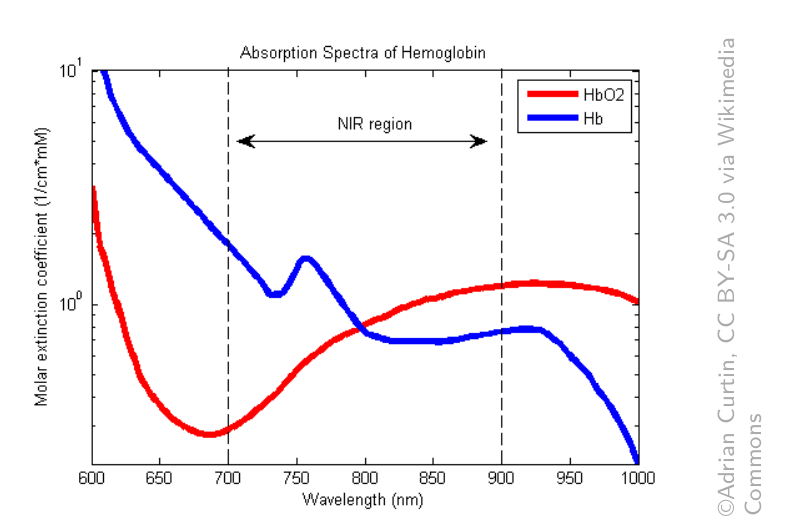
\includegraphics[width=0.7\textwidth]{../common/spectra.png}
		\caption{Absorption Spectra - Hb/HbO\textsubscript{2}}
		\label{fig:spectrum}
	\end{figure}
	
	
	\begin{figure}[ht!]
		\centering
		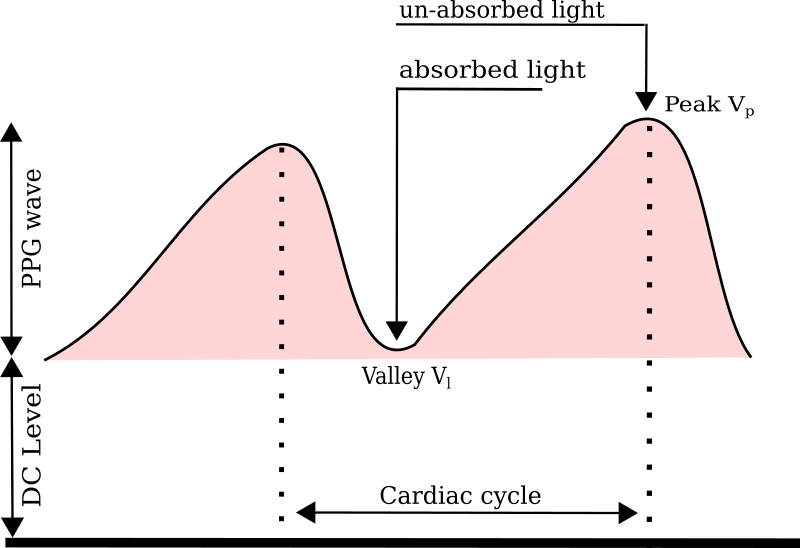
\includegraphics[width=0.7\textwidth]{images/PPG.png}
		\caption{PPG waveform when a single light source is projected}
		\label{fig:ppg}
	\end{figure}

	Heart pumps blood with each cardiac cycle and this leads to change in blood volume in the artery. When light is passed through (finger, earlobe, wrist\cite{light} depending on it's wavelength, Hb/HbO\textsubscript{2} components will also get absorbed and PPG signal is obtained as an output. Signal peaks correspond to completion of a cardiac cycle (heart beat). This varying signal also has a DC level due to absorption of light source by skin, venous blood and tissue.

	From this understanding, if we can find molecular concentrations of Hb and HbO\textsubscript{2} in a defined blood volume, SpO\textsubscript{2} can be calculated as a ratio of oxygenated blood concentration to total concentration: 

	\begin{equation}
		SpO\textsubscript{2} = \frac{HbO\textsubscript{2}}{Hb + 	HbO\textsubscript{2}}
	\end{equation}
	
	According to Beer-Lambert law:
	
	\begin{equation}		
		\log_{10}\frac{I}{I_o} = \epsilon l c
	\end{equation}	
	
	$I -$ Transmitted light intensity
	
	$I\textsubscript{o}-$ Incident light intensity
	
	$l -$ length
	
	$c -$ Molecular concentration
	
	$\epsilon -$ Molar absorption coefficient


	\begin{figure}[ht!]
		\centering
		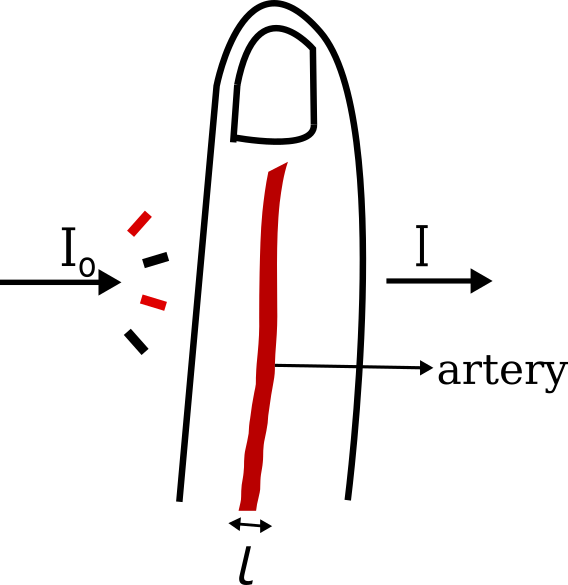
\includegraphics[width=0.3\textwidth]{images/finger_en.png}
		\caption{Light source projected onto a finger}
		\label{fig:finger}
	\end{figure}
	
	As seen in Figure \ref{fig:finger}, a light source is projected onto a finger and transmitted light is detected on the other end. Infrared and Red light is pulsed individually. For infrared source:
	
	\[	
	c_1 = 	\frac{\log_{10}\frac{I_1}{I_{o1}}}{\epsilon_1 l}
	\]	
	
	Since HbO\textsubscript{2} has higher absorption for infrared wavelength,

	\[	
	HbO_2 = \frac{\log_{10}\frac{I_1}{I_{o1}}}{\epsilon_1 	l}
	\]	
	
	Similarly for red,
	\[	
	Hb = \frac{\log_{10}\frac{I_2}{I_{o2}}}{\epsilon_2 	l}
	\]
	
	According to (1),

	\[	
	SpO_2 =  \frac{\frac{\log_{10}\frac{I_1}{I_{o1}}}{\epsilon_1 l}}		
	{\frac{\log_{10}\frac{I_2}{I_{o2}}}{\epsilon_2 l} + 	\frac{\log_{10}\frac{I_1}{I{o1}}}{\epsilon_1 l}}
	\]	
	
	if $R = \frac{\log_{10}\frac{I_2}{I_{o2}}}{\log_{10}\frac{I_1}{I_{o1}}}$,
	
	\[	
	SpO_2 = \frac{\frac{1}{\epsilon_1}}{\frac{R}{\epsilon_2} + \frac{1}{\epsilon_1}}
	\]	
	
	\begin{equation}
		SpO_2 = \frac{\epsilon_2}{R\epsilon_1 + \epsilon_2}
	\end{equation}	


	SpO\textsubscript{2} mostly depends on R, we can consider calculating R and later comparing with a calibrated reference to get the actual SpO\textsubscript{2}.
	
	Since Incident light intensity level would be constant while pulsed, R would depend only upon I\textsubscript{1} and I\textsubscript{2},

	\[
	R \approx \frac{\log_{10}{I_2}}{\log_{10}{I_1}} \approx \frac{I_2}{I_1} \approx \frac{AC_2}{AC_1}
	\]		
	
	We need not calculate the logarithm, as the actual SpO\textsubscript{2} would be obtained from a Look up table or an empirical equation which demonstrates relation of R to SpO\textsubscript{2}. Standard oximeter manufacturers would test their device on large group of subjects and obtain the R values and subject's actual SpO\textsubscript{2} using a separate calibrated meter to prepare a relationship curve. Once this mapping is obtained, SpO\textsubscript{2} for any subject can be calculated using the relationship.
	
	\begin{figure}[ht!]
	\centering	
	\begin{tikzpicture}
		\begin{axis}[
			xlabel = R,
			ylabel = SpO\textsubscript{2}\%]
			\addplot coordinates {
				(0.4, 100)
				(1, 85)
				(1.5, 72.5)
				(2, 60)
				(2.5, 47.5)
				(3, 35)
				(3.5, 22.5)
				(4, 10)
				(4.4,0)
			};
			
		\end{axis}
	\end{tikzpicture}
	\caption{A typical relationship curve R vs SpO\textsubscript{2}}
	\label{fig:curve}
	\end{figure}

	Since detected IR and Red signals can have varying DC levels, we need to normalize the ratio first by dividing the DC levels so that a direct comparison of the PPG (AC component) can be performed as that caries the absorbed/un-absorbed information, hence R now becomes:

	\[
		R = \sfrac{\frac{AC_2}{DC_2}}{{\frac{AC_1}{DC_1}}}
	\]	
	
	\begin{figure}[ht!]
		\centering
		\subfloat[Before Normalization
		]{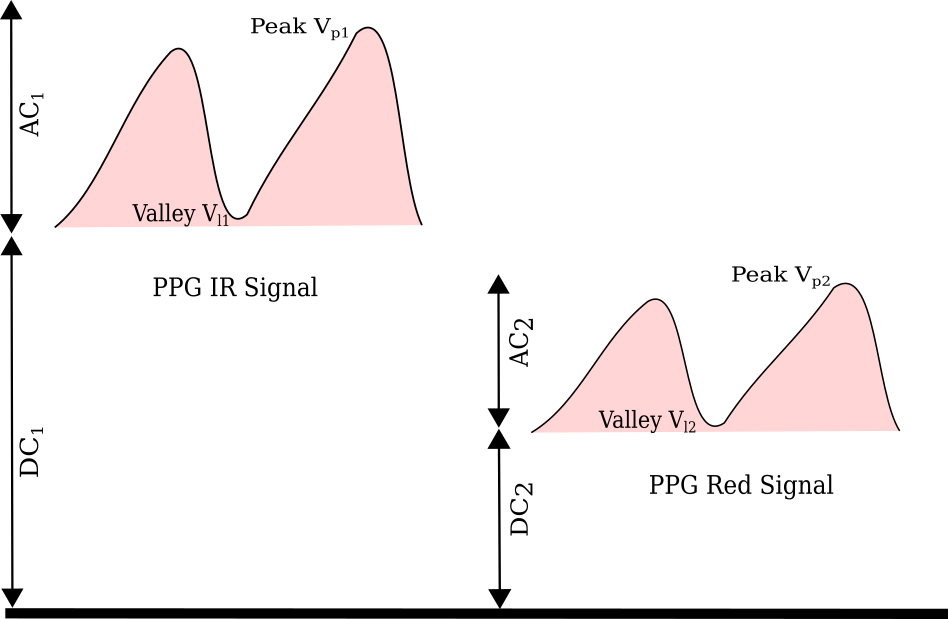
\includegraphics[width=0.7\textwidth]{images/PPG_norm1.png}}
		\hfill
		\subfloat[After Normalization
		]{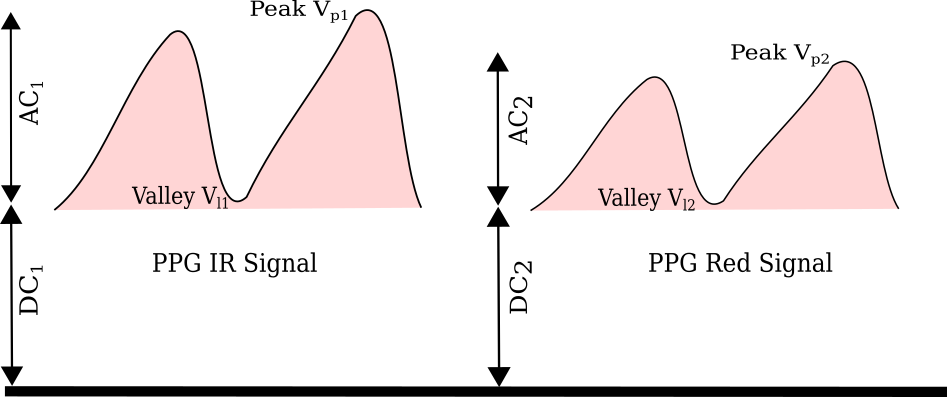
\includegraphics[width=0.7\textwidth]{images/PPG_norm2.png}}
		\caption{Effect of Normalization}
		\label{fig:ppgnorm}
	\end{figure}

	\begin{equation}
	\label{eq:calc}	
	R = \sfrac{\frac{V_{p2} - V_{l2}}{DC_2}}{\frac{V_{p1} - V_{l1}}{DC_1}}
	\end{equation}	 

	As shown in Figure \ref{fig:ppgnorm},
	
	$V_{p1} - $  Ir Peak
	
	$V_{l1} - $  Ir Valley
	
	$V_{p2} - $  Red Peak
	
	$V_{l2} - $  Red Valley
	
	$DC_1 - $  Ir DC level
	
	$DC_2 - $  Red DC level


	This value of R when compared with relationship curve would give the actual SpO\textsubscript{2}.
	
	We can consider calculating R for a set of samples and average them, instead of
	waiting for peaks and valleys to arrive. In this implementation, R is calculated between neighboring samples and a weighted average{\cite{wuk}} is calculated for final value. This is discussed further in SpO\textsubscript{2} calculation algorithm section.